\clearpage

\section{Sink}

\begin{tcolorbox}	
	\begin{tabular}{p{2.75cm} p{0.2cm} p{10.5cm}} 	
		\textbf{Header File}   &:& sink\_*.h \\
		\textbf{Source File}   &:& sink\_*.cpp \\
        \textbf{Version}       &:& 20180523 (Andr\'e Mourato)
	\end{tabular}
\end{tcolorbox}

This block accepts one input signal and it does not produce output signals. It takes samples out of the buffer until the buffer is empty. It has the option of displaying the number of samples still available.

\subsection*{Input Parameters}

\begin{table}[h]
	\centering
	\begin{tabular}{|c|c|p{30mm}|c|ccp{60mm}}
		\cline{1-4}
		\textbf{Parameter} & \textbf{Type} & \textbf{Values} &   \textbf{Default}& \\ \cline{1-4}
		numberOfSamples & long int & any & $-1$ \\ \cline{1-4}
        asciiFilePath & string & any & ``file\_output\_data.txt" \\ \cline{1-4}
        numberOfBitsToSkipBeforeSave & long int & non-negative & $0$ \\ \cline{1-4}
        numberOfBytesToSaveInFile & long int & non-negative & $0$ \\ \cline{1-4}
	\end{tabular}
	\caption{Sampler input parameters}
	\label{table:sink_in_par}
\end{table}

\subsection*{Methods}

Sink(vector$<$Signal *$>$ \&InputSig, vector$<$Signal *$>$ \&OutputSig)
\bigbreak
bool runBlock(void)
\bigbreak
void setAsciiFilePath(string newName)
\bigbreak
string getAsciiFilePath()
\bigbreak
void setNumberOfBitsToSkipBeforeSave(long int newValue)
\bigbreak
long int getNumberOfBitsToSkipBeforeSave()
\bigbreak
void setNumberOfBytesToSaveInFile(long int newValue)
\bigbreak
long int getNumberOfBytesToSaveInFile()
\bigbreak
void setNumberOfSamples(long int nOfSamples)
\bigbreak
void setDisplayNumberOfSamples(bool opt)

\subsection*{Functional Description} 
This block writes a signal to a file in the Ascii format. The path of the file is specified by the variable \textbf{asciiFilePath}.
Before saving the bits to a file, the \textbf{Sink} block will discard \textbf{numberOfBitsToSkipBeforeSave} bits. After this it will write \textbf{numberOfBytesToSaveInFile} bytes to the file. For this example we will use the binary signal shown in Figure \ref{fig:generatedoutputsignalfile}. This signal corresponds to the following bit stream: \textbf{0110000101100010} with zeros appended to the right. This bit stream is the concatenation of the ascii code of character \textbf{a} and character \textbf{b}, \textbf{01100001} and \textbf{01100010}, respectively. This means that, for the input parameters \textbf{numberOfBitsToSkipBeforeSave = 0} and \textbf{numberOfBytesToSaveInFile = 2} the content of \textbf{file\_output\_data.txt} will be: \textit{ab}


\begin{figure}[h]
	\centering
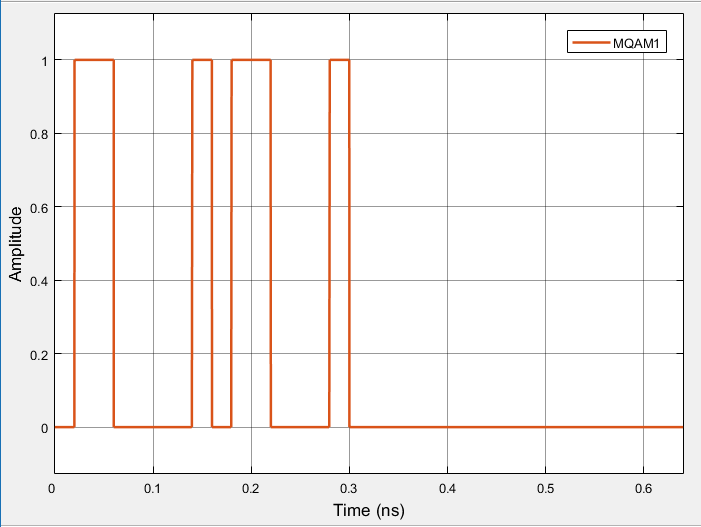
\includegraphics[width=.6\linewidth]{./lib/binary_source/figures/generated_signal_file}
\caption{The signal is generated according to the binary information of a file}\label{fig:generatedoutputsignalfile}
\end{figure}
